% TODO: falar das métricas e tipo "quanto menor melhor"

\slide{Escolha de Parâmetros}{
    \begin{itemize}
        \item Passado Visível: 4 horas;
        \item Tamanho do Intervalo de Fluxo: 2.5 minutos;
        \item Quantidade de Divisões: 4;
    \end{itemize}
}

\slide{Escolha do Passado Visível}{
     \begin{figure}[htbp]
        \centering
        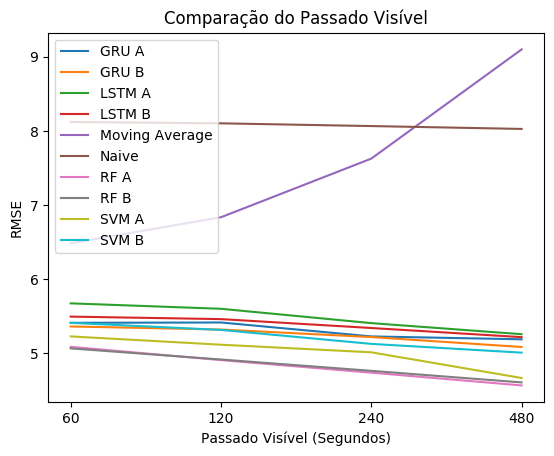
\includegraphics[scale=0.55]{monography/img/comparisons/comparacao_do_passado_visivel_rmse.png}
    \end{figure}
}

\slide{Escolha do Passado Visível (Tabela)}{
    \resizebox{\columnwidth}{100pt}{
        \begin{table}[htbp]
            \begin{tabular*}{\linewidth}{@{\extracolsep{\fill}}lllll}
            \toprule
             & 
            \multicolumn{1}{l}{\textbf{60}} & 
            \multicolumn{1}{l}{\textbf{120}} &
            \multicolumn{1}{l}{\textbf{240}} &
            \multicolumn{1}{l}{\textbf{480}} \\
            \midrule
            \textbf{MM} & \textbf{6.48} $\pm$ 0.62 & 6.83 $\pm$ 0.64 & 7.62 $\pm$ 0.68 & 9.09 $\pm$ 0.74
            \\
            \midrule
            \textbf{Naive} & 8.12 $\pm$ 0.86 & \textbf{8.10} $\pm$ 0.87 & 8.06 $\pm$ 0.88 & 8.02 $\pm$ 0.86 
            \\
            \midrule
            \textbf{RF A} & 5.08 $\pm$ 0.75 & 4.91 $\pm$ 0.73 & 4.74 $\pm$ 0.70 & \textbf{4.56} $\pm$ 0.73 
            \\
            \midrule
            \textbf{RF B} & 5.06 $\pm$ 0.75 & 4.91 $\pm$ 0.72 & 4.76 $\pm$ 0.70 & \textbf{4.61} $\pm$ 0.74 
            \\
            \midrule
            \textbf{SVM A} & 5.23 $\pm$ 0.70 & 5.11 $\pm$ 0.70 & 5.01 $\pm$ 0.69 & \textbf{4.66} $\pm$ 0.73 
            \\
            \midrule
            \textbf{SVM B} & 5.41 $\pm$ 0.62 & 5.31 $\pm$ 0.62 & 5.12 $\pm$ 0.58 & \textbf{5.01} $\pm$ 0.61 
            \\
            \midrule
            \textbf{LSTM A} & 5.67 $\pm$ 0.81 & 5.60 $\pm$ 0.71 & 5.40 $\pm$ 0.75 & \textbf{5.26} $\pm$ 0.76 
            \\
            \midrule
            \textbf{LSTM B} & 5.49 $\pm$ 0.56 & 5.46 $\pm$ 0.57 & 5.34 $\pm$ 0.73 & \textbf{5.22} $\pm$ 0.76 
            \\
            \midrule
            \textbf{GRU A} & 5.41 $\pm$ 0.70 & 5.41 $\pm$ 0.65 & 5.23 $\pm$ 0.61 & \textbf{5.19} $\pm$ 0.74 
            \\
            \midrule
            \textbf{GRU B} & 5.36 $\pm$ 0.63 & 5.32 $\pm$ 0.71 & 5.22 $\pm$ 0.74 & \textbf{5.08} $\pm$ 0.67
            \\
            \bottomrule
            \end{tabular*}
        \end{table}
    }
}

\slide{Tamanho do Intervalo do Fluxo}{
     \begin{figure}[H]
        \centering
        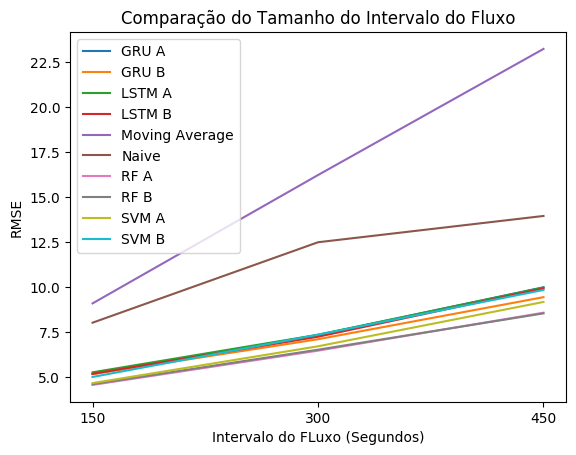
\includegraphics[scale=0.55]{monography/img/comparisons/comparacao_do_tamanho_do_intervalo_do_fluxo_rmse.png}
    \end{figure}
}

\slide{Tamanho do Intervalo do Fluxo (Tabela)}{
    \resizebox{\columnwidth}{100pt}{%
        \begin{table}[H]
            \begin{tabular*}{\linewidth}{@{\extracolsep{\fill}}llll}
            \toprule
             & 
            \multicolumn{1}{l}{\textbf{150}} & 
            \multicolumn{1}{l}{\textbf{300}} &
            \multicolumn{1}{l}{\textbf{450}} \\
            \midrule
            \textbf{MM} & \textbf{9.09} $\pm$ 0.74 & 16.22 $\pm$ 0.87 & 23.23 $\pm$ 1.45
            \\
            \midrule
            \textbf{Naive} & \textbf{8.02} $\pm$ 0.86 & 12.49 $\pm$ 2.05 & 13.95 $\pm$ 1.67
            \\
            \midrule
            \textbf{RF A} & \textbf{4.56} $\pm$ 0.73 & 6.47 $\pm$ 0.46 & 8.58 $\pm$ 1.41
            \\
            \midrule
            \textbf{RF B} & \textbf{4.61} $\pm$ 0.74 & 6.52 $\pm$ 0.38 & 8.54 $\pm$ 1.22
            \\
            \midrule
            \textbf{SVM A} & \textbf{4.66} $\pm$ 0.73 & 6.71 $\pm$ 0.32 & 9.17 $\pm$ 0.95
            \\
            \midrule
            \textbf{SVM B} & \textbf{5.01} $\pm$ 0.61 & 7.36 $\pm$ 0.38 & 9.84 $\pm$ 0.36
            \\
            \midrule
            \textbf{LSTM A} & \textbf{5.26} $\pm$ 0.80 & 7.35 $\pm$ 0.60 & 9.97 $\pm$ 0.80
            \\
            \midrule
            \textbf{LSTM B} & \textbf{5.18} $\pm$ 0.71 & 7.24 $\pm$ 0.63 & 9.92 $\pm$ 0.98
            \\
            \midrule
            \textbf{GRU A} & \textbf{5.18} $\pm$ 0.67 & 7.33 $\pm$ 0.60 & 9.99 $\pm$ 1.03
            \\
            \midrule
            \textbf{GRU B} & \textbf{5.16} $\pm$ 0.75 & 7.10 $\pm$ 0.66 & 9.44 $\pm$ 1.52
            \\
            \bottomrule
            \end{tabular*}
        \end{table} 
    }
}

\slide{Número de Divisões do Conjunto de Dados}{
     \begin{figure}[H]
        \centering
        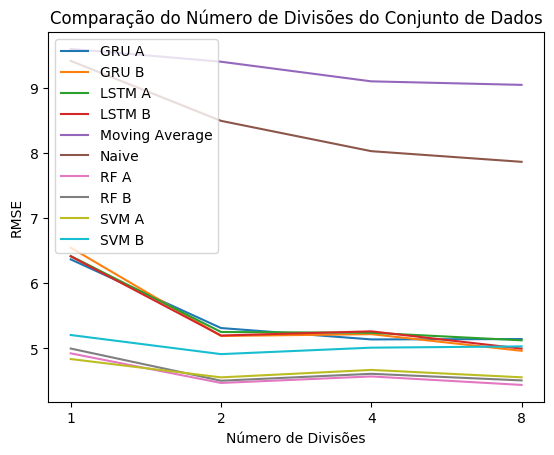
\includegraphics[scale=0.55]{monography/img/comparisons/comparacao_do_numero_de_divisoes_do_conjunto_de_dados_rmse.png}
    \end{figure}
}

\slide{Número de Divisões do Conjunto de Dados (Tabela)}{
    \resizebox{\columnwidth}{100pt}{%
        \begin{table}[htbp]
            \begin{tabular*}{\linewidth}{@{\extracolsep{\fill}}lllll}
            \toprule
             & 
            \multicolumn{1}{l}{\textbf{1}} & 
            \multicolumn{1}{l}{\textbf{2}} &
            \multicolumn{1}{l}{\textbf{4}} &
            \multicolumn{1}{l}{\textbf{8}} \\
            \midrule
            \textbf{MM} & 9.59 $\pm$ 0.00 & 9.39 $\pm$ 0.00 & 9.09 $\pm$ 0.74 & \textbf{9.04} $\pm$ 0.88
            \\
            \midrule
            \textbf{Naive} & 9.41 $\pm$ 0.00 & 8.49 $\pm$ 0.77 & 8.02 $\pm$ 0.86 & \textbf{7.86} $\pm$ 0.88
            \\
            \midrule
            \textbf{RF A} & 4.92 $\pm$ 0.00 & 4.46 $\pm$ 0.25 & 4.56 $\pm$ 0.73 & \textbf{4.43} $\pm$ 0.51
            \\
            \midrule
            \textbf{RF B} & 4.99 $\pm$ 0.00 & 4.50 $\pm$ 0.24 & 4.61 $\pm$ 0.74 & \textbf{4.50} $\pm$ 0.50
            \\
            \midrule
            \textbf{SVM A} & 4.83 $\pm$ 0.00 & \textbf{4.55} $\pm$ 0.16 & 4.66 $\pm$ 0.73 & 4.55 $\pm$ 0.49
            \\
            \midrule
            \textbf{SVM B} & 5.20 $\pm$ 0.00 & \textbf{4.91} $\pm$ 0.04 & 5.01 $\pm$ 0.61 & 5.03 $\pm$ 0.51
            \\
            \midrule
            \textbf{LSTM A} & 6.41 $\pm$ 0.00 & 5.25 $\pm$ 0.27 & 5.23 $\pm$ 0.79 & \textbf{5.12} $\pm$ 0.67
            \\
            \midrule
            \textbf{LSTM B} & 6.41 $\pm$ 0.00 & 5.19 $\pm$ 0.15 & 5.26 $\pm$ 0.83 & \textbf{4.99} $\pm$ 0.69
            \\
            \midrule
            \textbf{GRU A} & 6.36 $\pm$ 0.00 & 5.31 $\pm$ 0.01 & \textbf{5.13} $\pm$ 0.70 & 5.14 $\pm$ 0.51
            \\
            \midrule
            \textbf{GRU B} & 6.54 $\pm$ 0.00 & 5.19 $\pm$ 0.03 & 5.21 $\pm$ 0.68 & \textbf{4.96} $\pm$ 0.64
            \\
            \bottomrule
            \end{tabular*}
        \end{table}
    }
}

\slide{Resultado antes do \textit{Tuning}}{
     \begin{figure}[H]
        \centering
        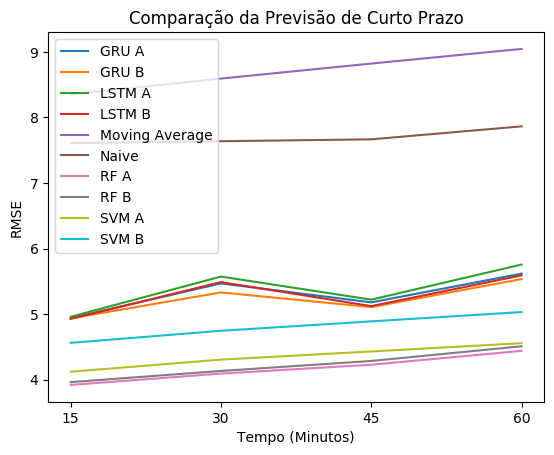
\includegraphics[scale=0.55]{monography/img/comparisons/comparacao_da_previsao_de_curto_prazo_rmse.png}
    \end{figure}
}

\slide{Resultado antes do \textit{Tuning} (Tabela)}{
     \resizebox{\columnwidth}{100pt}{%
        \begin{table}[H]
            \begin{tabular*}{\linewidth}{@{\extracolsep{\fill}}lllll}
            \toprule
             & 
            \multicolumn{1}{l}{\textbf{15 mins}} & 
            \multicolumn{1}{l}{\textbf{30 mins}} &
            \multicolumn{1}{l}{\textbf{45 mins}} &
            \multicolumn{1}{l}{\textbf{60 mins}} \\
            \midrule
            \textbf{MM} & 8.35 $\pm$ 0.82 & 8.59 $\pm$ 0.84 & 8.82 $\pm$ 0.86 & 9.04 $\pm$ 0.88
            \\
            
            \midrule
            \textbf{Naive} & 7.60 $\pm$ 0.99 & 7.63 $\pm$ 0.83 & 7.66 $\pm$ 0.76 & 7.86 $\pm$ 0.88
            \\
            
            \midrule
            \textbf{RF A} & \textcolor{blue}{\textbf{3.91 $\pm$ 0.39}} & \textcolor{blue}{\textbf{4.09 $\pm$ 0.40}} & \textcolor{blue}{\textbf{4.22 $\pm$ 0.46}} & \textcolor{blue}{\textbf{4.43 $\pm$ 0.51}}
            \\
            
            \midrule
            \textbf{RF B} & 3.96 $\pm$ 0.40 & 4.13 $\pm$ 0.41 & 4.28 $\pm$ 0.46 & 4.50 $\pm$ 0.50
            \\
            
            \midrule
            \textbf{SVM A} & 4.12 $\pm$ 0.45 & 4.30 $\pm$ 0.46 & 4.42 $\pm$ 0.49 & 4.55 $\pm$ 0.49
            \\
            
            \midrule
            \textbf{SVM B} & 4.56 $\pm$ 0.46 & 4.74 $\pm$ 0.47 & 4.88 $\pm$ 0.50 & 5.03 $\pm$ 0.51
            \\
            
            \midrule
            \textbf{LSTM A} & 4.95 $\pm$ 0.57 & 5.57 $\pm$ 0.53 & 5.21 $\pm$ 0.52 & 5.75 $\pm$ 0.44
            \\
            
            \midrule
            \textbf{LSTM B} & 4.92 $\pm$ 0.56 & 5.48 $\pm$ 0.57 & 5.12 $\pm$ 0.58 & 5.59 $\pm$ 0.59
            \\
            
            \midrule
            \textbf{GRU A} & 4.93 $\pm$ 0.57 & 5.46 $\pm$ 0.54 & 5.17 $\pm$ 0.58 & 5.61 $\pm$ 0.53
            \\
            
            \midrule
            \textbf{GRU B} & 4.93 $\pm$ 0.62 & 5.33 $\pm$ 0.47 & 5.10 $\pm$ 0.61 & 5.53 $\pm$ 0.54
            \\
            \bottomrule
            \end{tabular*}
        \end{table}
     }
}

\slide{Resultado depois do \textit{Tuning}}{
     \begin{figure}[H]
        \centering
        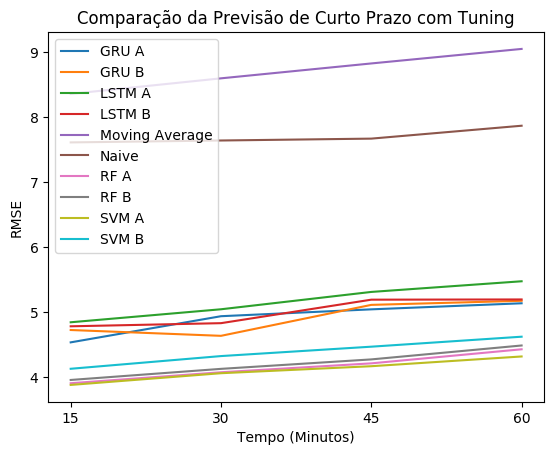
\includegraphics[scale=0.55]{monography/img/comparisons/comparacao_da_previsao_de_curto_prazo_com_tuning_rmse.png}
    \end{figure}
}

\slide{Resultado depois do \textit{Tuning} (Tabela)}{
     \resizebox{\columnwidth}{100pt}{%
        
        \begin{table}[H]
            \begin{tabular*}{\linewidth}{@{\extracolsep{\fill}}lllll}
            \toprule
             & 
            \multicolumn{1}{l}{\textbf{15 mins}} & 
            \multicolumn{1}{l}{\textbf{30 mins}} &
            \multicolumn{1}{l}{\textbf{45 mins}} &
            \multicolumn{1}{l}{\textbf{60 mins}} \\
            \midrule
            \textbf{MM} & 8.35 $\pm$ 0.82 & 8.59 $\pm$ 0.84 & 8.82 $\pm$ 0.86 & 9.04 $\pm$ 0.88
            \\
            \midrule
            \textbf{Naive} & 7.60 $\pm$ 0.99 & 7.63 $\pm$ 0.83 & 7.66 $\pm$ 0.76 & 7.86 $\pm$ 0.88
            \\
            \midrule
            \textbf{RF A} & 3.90 $\pm$ 0.39 & 4.07 $\pm$ 0.42 & 4.21 $\pm$ 0.46 & 4.42 $\pm$ 0.51
            \\
            \midrule
            \textbf{RF B} & 3.95 $\pm$ 0.39 & 4.12 $\pm$ 0.40 & 4.27 $\pm$ 0.47 & 4.48 $\pm$ 0.50
            \\
            \midrule
            \textbf{SVM A} &  \textcolor{blue}{\textbf{3.87} $\pm$}  \textcolor{blue}{\textbf{0.42}} & \textcolor{blue}{\textbf{4.05 $\pm$ 0.44}} & \textcolor{blue}{\textbf{4.16 $\pm$ 0.48}} & \textcolor{blue}{\textbf{4.31 $\pm$ 0.53}}
            \\
            \midrule
            \textbf{SVM B} & 4.12 $\pm$ 0.33 & 4.32 $\pm$ 0.38 & 4.46 $\pm$ 0.46 & 4.61 $\pm$ 0.52
            \\
            \midrule
            \textbf{LSTM A} & 4.84 $\pm$ 0.62 & 5.04 $\pm$ 0.53 & 5.30 $\pm$ 0.37 & 5.47 $\pm$ 0.50
            \\
            \midrule
            \textbf{LSTM B} & 4.77 $\pm$ 0.56 & 4.82 $\pm$ 0.55 & 5.18 $\pm$ 0.60 & 5.19 $\pm$ 0.69
            \\
            \midrule
            \textbf{GRU A} & 4.53 $\pm$ 0.55 & 4.93 $\pm$ 0.30 & 5.04 $\pm$ 0.53 & 5.13 $\pm$ 0.48
            \\
            \midrule
            \textbf{GRU B} & 4.72 $\pm$ 0.67 & 4.63 $\pm$ 0.42 & 5.10 $\pm$ 0.66 & 5.17 $\pm$ 0.53
            \\
            \bottomrule
            \end{tabular*}
        \end{table}

    }
}

\slide{Análise de Hiper-parâmetros}{
\begin{table}[H]
    \begin{tabular*}{\linewidth}{@{\extracolsep{\fill}}lll}
    \toprule
     & 
    \multicolumn{1}{l}{\textbf{Taxa de Aprendizagem}} & 
    \multicolumn{1}{l}{\textbf{Células}} 
    \\
\midrule
\textbf{LSTM A} & 0.004 & 50\\ \midrule
\textbf{LSTM B} & 0.004 & 125 \\ \midrule
\textbf{GRU A} & 0.016 &  75 \\ \midrule
\textbf{GRU B} & 0.008 &  125 \\
    \bottomrule
    \end{tabular*}
    \label{table:best_hiper_deep}
    \caption{Valores de hiper-parâmetros mais recorrentes no \textit{Grid Search} para os modelos de aprendizagem profunda.}
\end{table}
}

\slide{Análise de Hiper-parâmetros}{
\begin{table}[H]
    \begin{tabular*}{\linewidth}{@{\extracolsep{\fill}}lll}
    \toprule
     & 
    \multicolumn{1}{l}{\textbf{C}} & 
    \multicolumn{1}{l}{\textbf{Gamma}} 
    \\
\midrule
\textbf{SVM A} & 10 & scale\\ \midrule
\textbf{SVM B} & 100 & scale \\ \midrule

    \bottomrule
    \end{tabular*}
    \label{table:best_hiper_svm}
    \caption{Valores de hiper-parâmetros mais recorrentes no \textit{Grid Search} para o \textit{\acrshort{SVM}}}
\end{table}
}

\slide{Análise de Hiper-parâmetros}{
\begin{table}[H]
    \begin{tabular*}{\linewidth}{@{\extracolsep{\fill}}lll}
    \toprule
     & 
    \multicolumn{1}{l}{\textbf{Altura Máx. Arvore}} & 
    \multicolumn{1}{l}{\textbf{Nr. Estimadores}} 
    \\
\midrule
\textbf{RF A} & 32 & 800\\ \midrule
\textbf{RF B} & 32 & 800 \\ \midrule

    \bottomrule
    \end{tabular*}
    \label{table:best_hiper_rf}
    \caption{Valores de hiper-parâmetros mais recorrentes no \textit{Grid Search} para o \textit{\acrshort{RF}}.}
\end{table}
}

\slide{Observações}{
     \begin{itemize}
         \item Os resultados utilizando a métrica \textbf{MAE} foram muito similares ao resultados com \textbf{RMSE};
         \item Com a métrica \(\alpha\), os modelos apresentaram uma acurácia próxima de 60\%, no qual o \textit{SVM} e \textit{RF} apresentaram uma acurácia de 70\% em alguns casos.
     \end{itemize}
}
